\documentclass[11pt]{article}
\usepackage[textwidth=18.0cm, textheight=23.0cm, top=2.0cm]{geometry}
\usepackage{pst-all}
\usepackage{amssymb}
\usepackage{tikz}
\usepackage{underscore}\begin{document}
\pagestyle{empty}


ClassName: \underline{\textbf{Class_04.2bp-13}}
\par
BinSize: \underline{\textbf{100 × 100}}
\par
ReduceSize: \underline{\textbf{100 × 100}}
\par
TypeNum: \underline{\textbf{40}}
\par
Num: \underline{\textbf{40}}
\par
OutS: \underline{\textbf{20000}}
\par
InS: \underline{\textbf{13176}}
\par
Rate: \underline{\textbf{0.659}}
\par
UB: \underline{\textbf{2}}
\par
LB0: \underline{\textbf{2}}
\par
LB: \underline{\textbf{2}}
\par
LBWithCut: \underline{\textbf{2}}
\par
NodeCut: \underline{\textbf{0}}
\par
ExtendedNodeCnt: \underline{\textbf{1}}
\par
GenNodeCnt: \underline{\textbf{1}}
\par
PrimalNode: \underline{\textbf{0}}
\par
ColumnCount: \underline{\textbf{2}}
\par
TotalCutCount: \underline{\textbf{0}}
\par
RootCutCount: \underline{\textbf{0}}
\par
LPSolverCnt: \underline{\textbf{1}}
\par
PricingSolverCnt: \underline{\textbf{0}}
\par
BranchAndBoundNum: \underline{\textbf{1}}
\par
isOpt: \underline{\textbf{true}}
\par
TimeOnInitSolution: \underline{\textbf{600.000 s}}
\par
TimeOnPrimal: \underline{\textbf{0.000 s}}
\par
TimeOnPricing: \underline{\textbf{0.000 s}}
\par
TimeOnRmp: \underline{\textbf{0.063 s}}
\par
TotalTime: \underline{\textbf{600.328 s}}
\par
\newpage


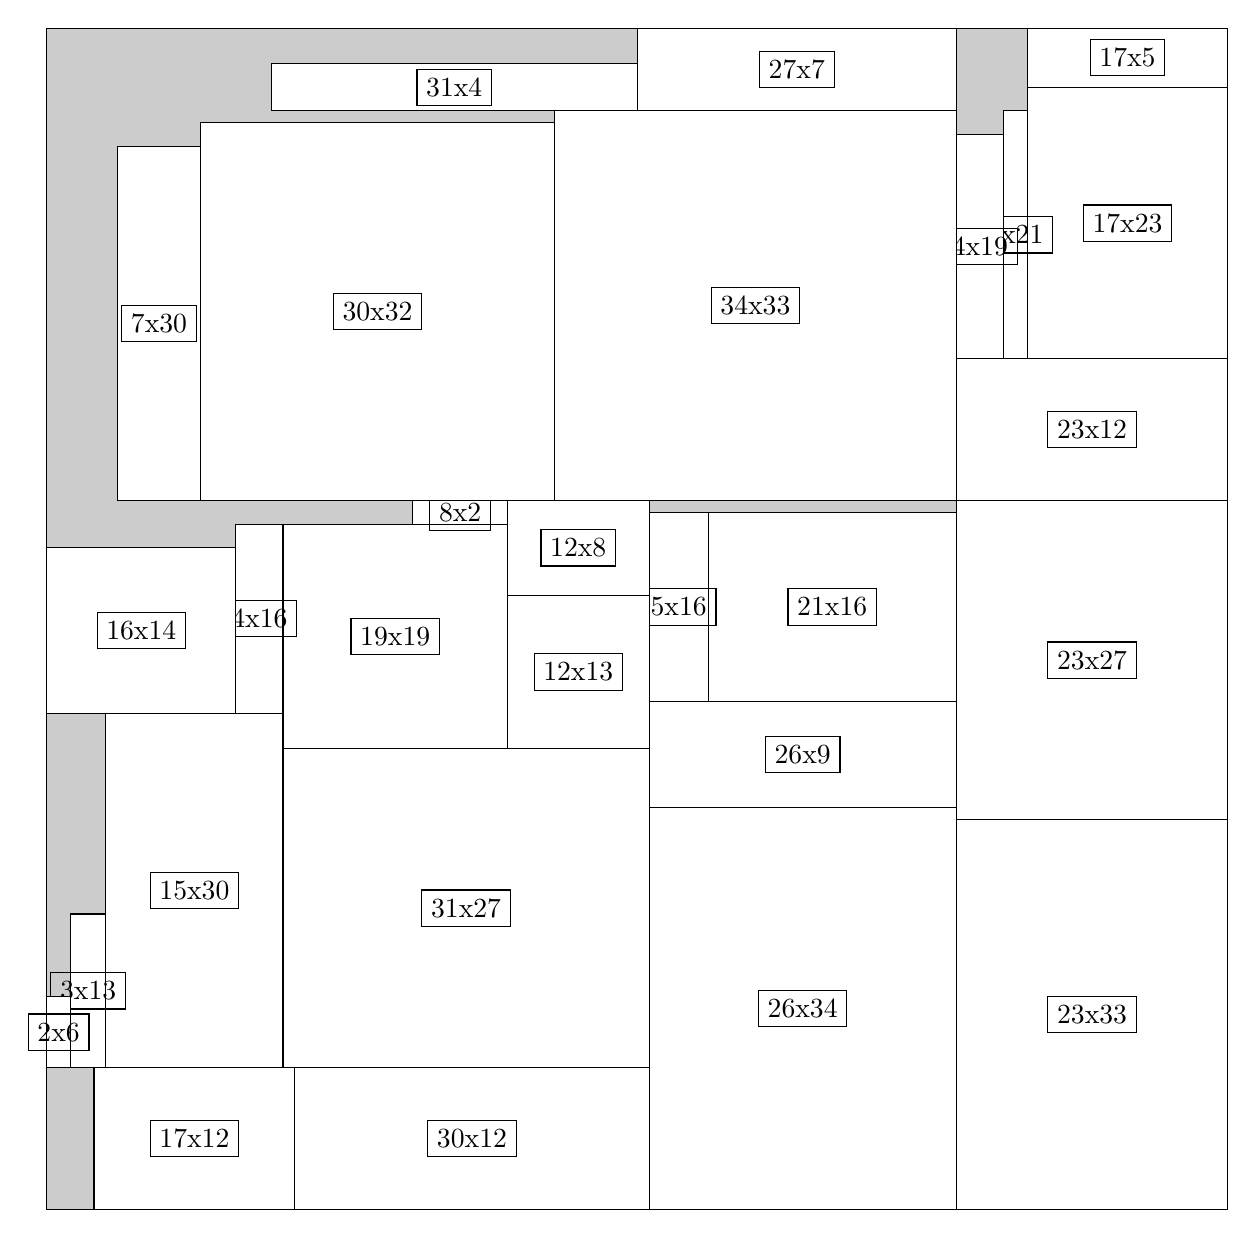
\begin{tikzpicture}[shorten >=1pt,scale=1.0,every node/.style={scale=1.0},->]
\tikzstyle{vertex}=[circle,fill=black!25,minimum size=14pt,inner sep=0pt]
\filldraw[fill=gray!40!white, draw=black] (0,0) rectangle (15.0,15.0);
\foreach \name/\x/\y/\w/\h in {23x33/11.549999999999999/0.0/3.4499999999999997/4.95,23x27/11.549999999999999/4.95/3.4499999999999997/4.05,23x12/11.549999999999999/9.0/3.4499999999999997/1.7999999999999998,17x23/12.45/10.799999999999999/2.55/3.4499999999999997,2x21/12.15/10.799999999999999/0.3/3.15,4x19/11.549999999999999/10.799999999999999/0.6/2.85,17x5/12.45/14.25/2.55/0.75,26x34/7.6499999999999995/0.0/3.9/5.1,26x9/7.6499999999999995/5.1/3.9/1.3499999999999999,21x16/8.4/6.45/3.15/2.4,5x16/7.6499999999999995/6.45/0.75/2.4,30x12/3.15/0.0/4.5/1.7999999999999998,17x12/0.6/0.0/2.55/1.7999999999999998,31x27/3.0/1.7999999999999998/4.6499999999999995/4.05,12x13/5.85/5.85/1.7999999999999998/1.95,12x8/5.85/7.8/1.7999999999999998/1.2,19x19/3.0/5.85/2.85/2.85,8x2/4.6499999999999995/8.7/1.2/0.3,15x30/0.75/1.7999999999999998/2.25/4.5,3x13/0.3/1.7999999999999998/0.44999999999999996/1.95,2x6/0.0/1.7999999999999998/0.3/0.8999999999999999,4x16/2.4/6.3/0.6/2.4,16x14/0.0/6.3/2.4/2.1,34x33/6.45/9.0/5.1/4.95,30x32/1.95/9.0/4.5/4.8,7x30/0.8999999999999999/9.0/1.05/4.5,27x7/7.5/13.95/4.05/1.05,31x4/2.85/13.95/4.6499999999999995/0.6}
\filldraw[fill=white!40!white, draw=black] (\x,\y) rectangle node[draw] (\name) {\name} ++(\w,\h);
\end{tikzpicture}


w =23 , h =33 , x =77 , y =0 , v =759
\par
w =23 , h =27 , x =77 , y =33 , v =621
\par
w =23 , h =12 , x =77 , y =60 , v =276
\par
w =17 , h =23 , x =83 , y =72 , v =391
\par
w =2 , h =21 , x =81 , y =72 , v =42
\par
w =4 , h =19 , x =77 , y =72 , v =76
\par
w =17 , h =5 , x =83 , y =95 , v =85
\par
w =26 , h =34 , x =51 , y =0 , v =884
\par
w =26 , h =9 , x =51 , y =34 , v =234
\par
w =21 , h =16 , x =56 , y =43 , v =336
\par
w =5 , h =16 , x =51 , y =43 , v =80
\par
w =30 , h =12 , x =21 , y =0 , v =360
\par
w =17 , h =12 , x =4 , y =0 , v =204
\par
w =31 , h =27 , x =20 , y =12 , v =837
\par
w =12 , h =13 , x =39 , y =39 , v =156
\par
w =12 , h =8 , x =39 , y =52 , v =96
\par
w =19 , h =19 , x =20 , y =39 , v =361
\par
w =8 , h =2 , x =31 , y =58 , v =16
\par
w =15 , h =30 , x =5 , y =12 , v =450
\par
w =3 , h =13 , x =2 , y =12 , v =39
\par
w =2 , h =6 , x =0 , y =12 , v =12
\par
w =4 , h =16 , x =16 , y =42 , v =64
\par
w =16 , h =14 , x =0 , y =42 , v =224
\par
w =34 , h =33 , x =43 , y =60 , v =1122
\par
w =30 , h =32 , x =13 , y =60 , v =960
\par
w =7 , h =30 , x =6 , y =60 , v =210
\par
w =27 , h =7 , x =50 , y =93 , v =189
\par
w =31 , h =4 , x =19 , y =93 , v =124
\par
\newpage


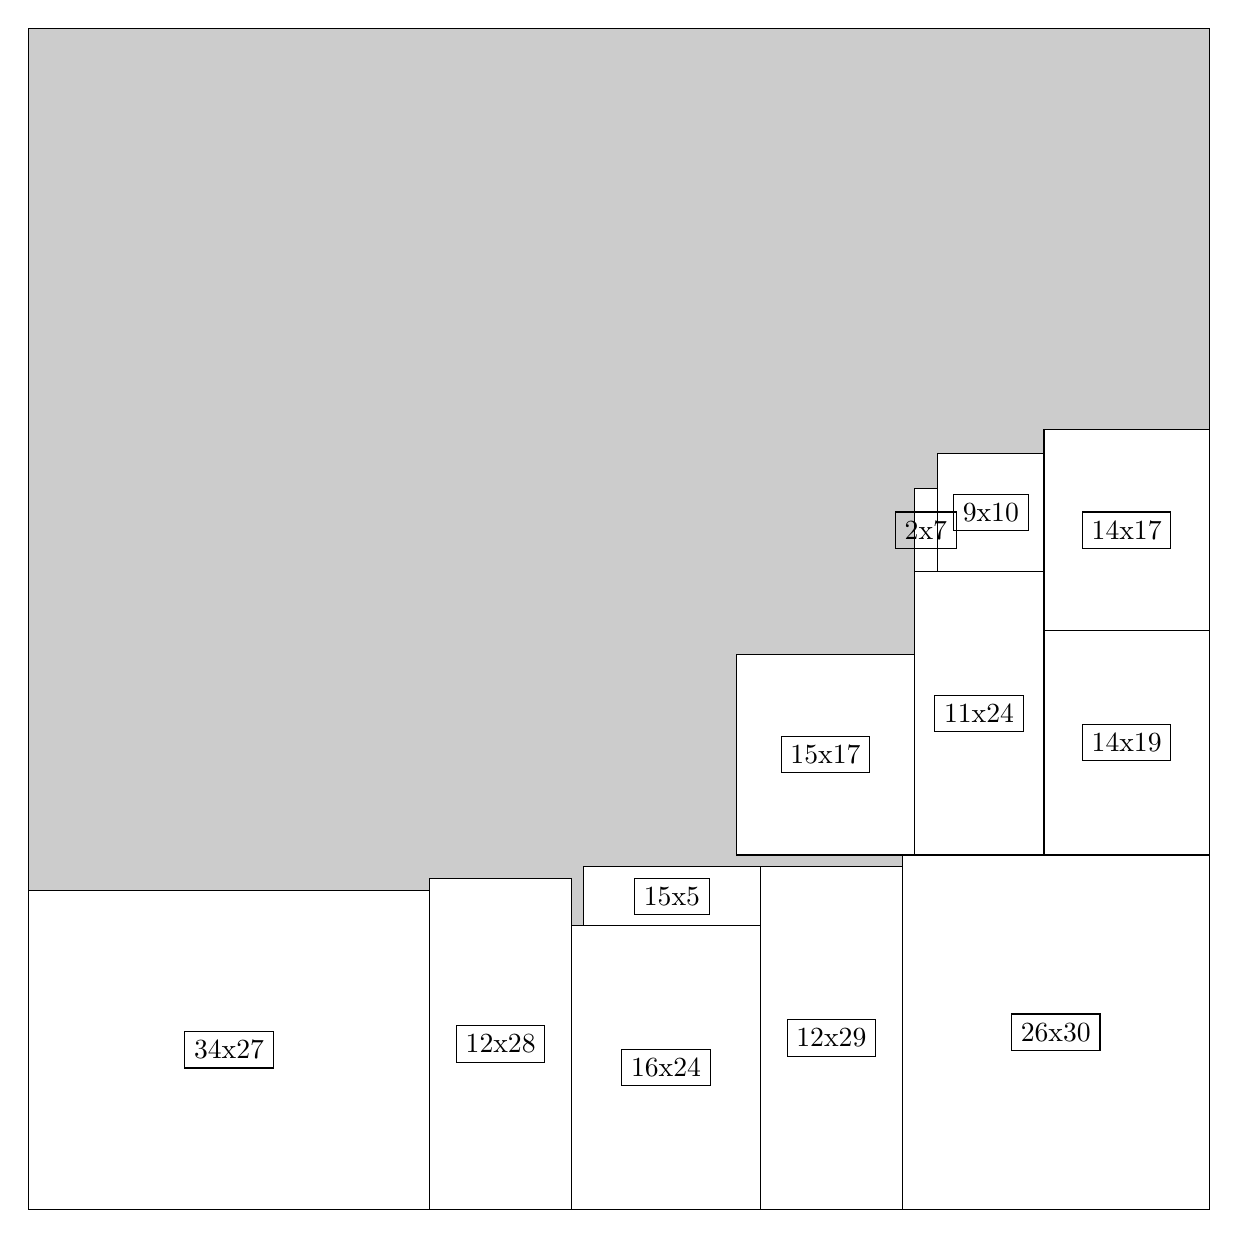
\begin{tikzpicture}[shorten >=1pt,scale=1.0,every node/.style={scale=1.0},->]
\tikzstyle{vertex}=[circle,fill=black!25,minimum size=14pt,inner sep=0pt]
\filldraw[fill=gray!40!white, draw=black] (0,0) rectangle (15.0,15.0);
\foreach \name/\x/\y/\w/\h in {26x30/11.1/0.0/3.9/4.5,12x29/9.299999999999999/0.0/1.7999999999999998/4.35,16x24/6.8999999999999995/0.0/2.4/3.5999999999999996,15x5/7.05/3.5999999999999996/2.25/0.75,12x28/5.1/0.0/1.7999999999999998/4.2,34x27/0.0/0.0/5.1/4.05,14x19/12.9/4.5/2.1/2.85,14x17/12.9/7.35/2.1/2.55,11x24/11.25/4.5/1.65/3.5999999999999996,9x10/11.549999999999999/8.1/1.3499999999999999/1.5,2x7/11.25/8.1/0.3/1.05,15x17/9.0/4.5/2.25/2.55}
\filldraw[fill=white!40!white, draw=black] (\x,\y) rectangle node[draw] (\name) {\name} ++(\w,\h);
\end{tikzpicture}


w =26 , h =30 , x =74 , y =0 , v =780
\par
w =12 , h =29 , x =62 , y =0 , v =348
\par
w =16 , h =24 , x =46 , y =0 , v =384
\par
w =15 , h =5 , x =47 , y =24 , v =75
\par
w =12 , h =28 , x =34 , y =0 , v =336
\par
w =34 , h =27 , x =0 , y =0 , v =918
\par
w =14 , h =19 , x =86 , y =30 , v =266
\par
w =14 , h =17 , x =86 , y =49 , v =238
\par
w =11 , h =24 , x =75 , y =30 , v =264
\par
w =9 , h =10 , x =77 , y =54 , v =90
\par
w =2 , h =7 , x =75 , y =54 , v =14
\par
w =15 , h =17 , x =60 , y =30 , v =255
\par
\newpage


\end{document}